\section{Desarrollo/Análisis}

Inicialmente se hizo la prueba del giroscopio para determinar que los 3 ejes funcionaran correctamente a la hora de mover la placa.
\begin{figure}[H]
\centering
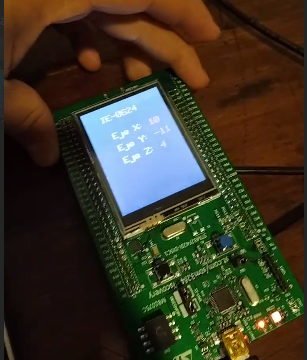
\includegraphics[width=.55\linewidth]{Imagenes/5.png}
 \caption{Funcionamiento del giroscopio.}
 \label{fig_gyro}
\end{figure}
Lo anterior se logró gracias los ejemplos dados de la biblioteca libopencm3. Y realizando otro tipo de depuraciones para darle un estilo a la presentación en la pantalla LCD.\par
Lo siguiente que se hizo fue la configuración de los GPIO's y establecer el pin \texttt{PA0} como entrada analógico y poder mostrar la tensión que posee la batería en el momento que es conectada. Inicialmente se hizo un divisor de tensión a partir de $v_{in}=\SI{9}{\volt}$, junto con resistencias de \SI{1.8}{\kilo\ohm} y \SI{1}{\kilo\ohm}, obtiendo una tensión de \SI{3.2}{\volt} tal como se muestra a continuación.
\begin{figure}[H]
\centering
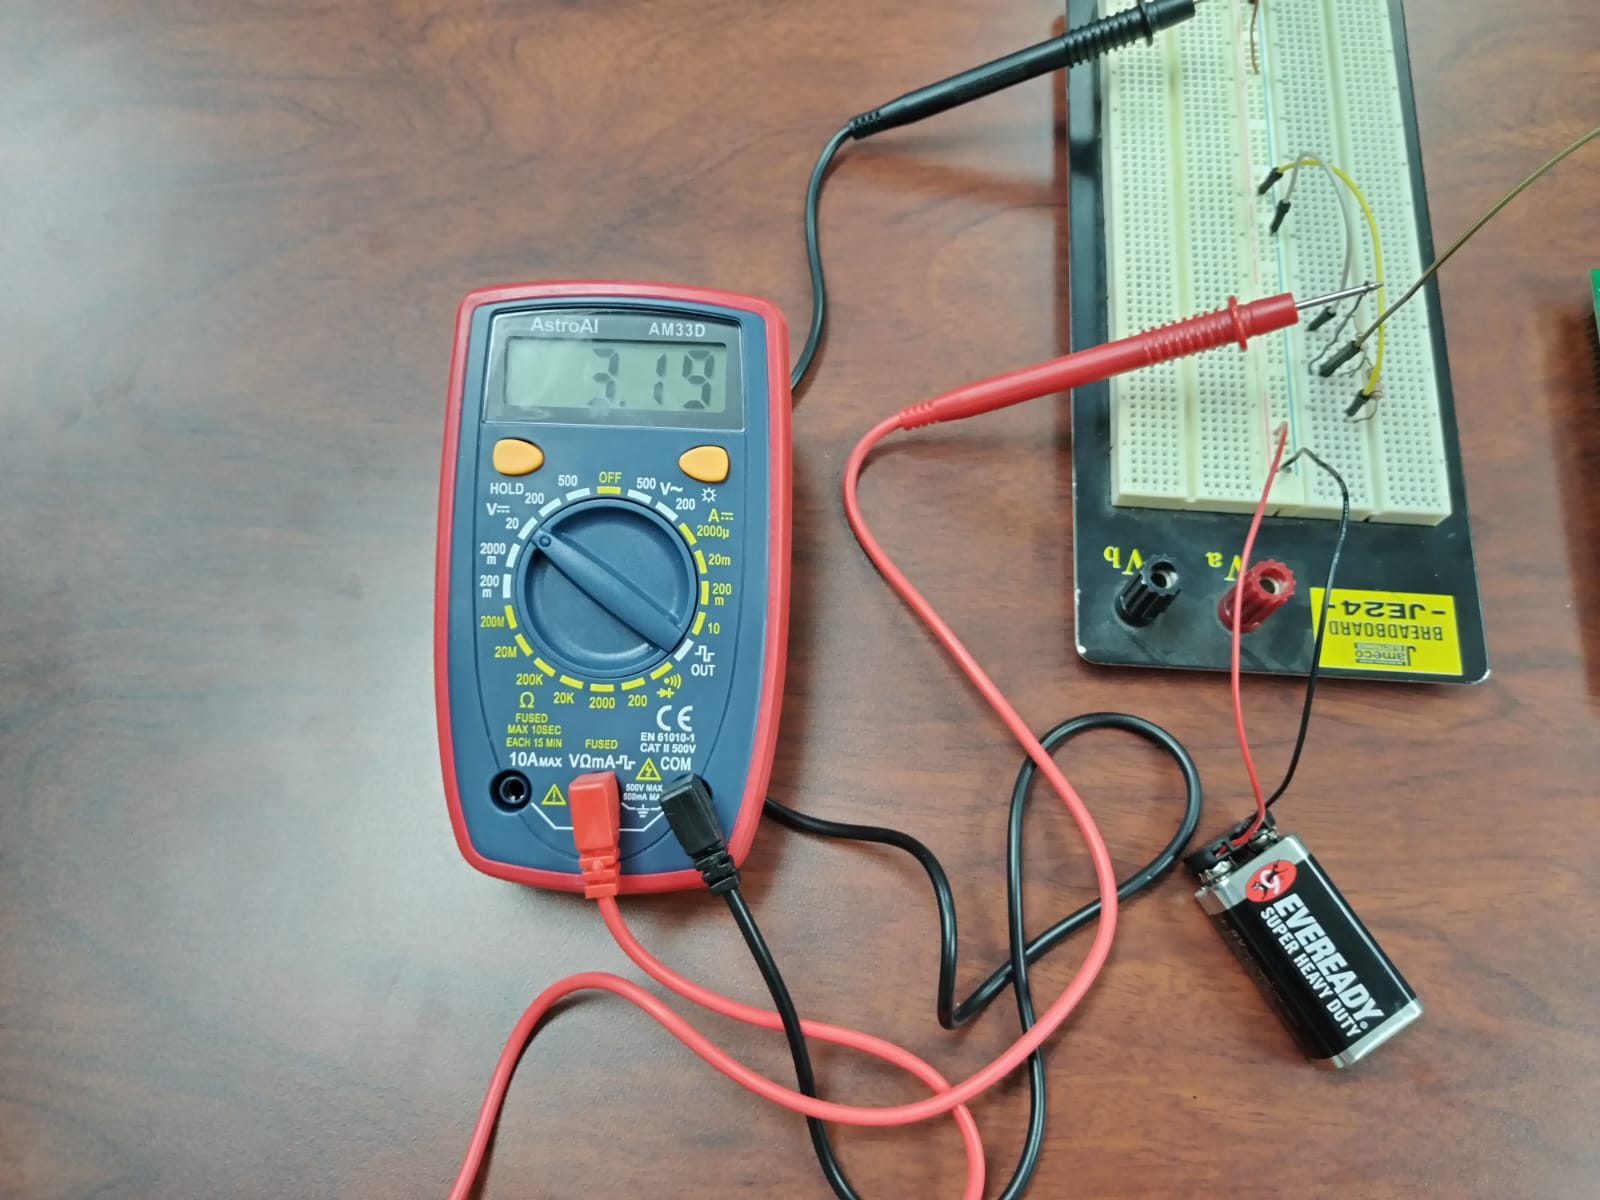
\includegraphics[width=.55\linewidth]{Imagenes/6.jpeg}
 \caption{Tensión de salida}
 \label{fig_vout}
\end{figure}
Esta tensión eléctrica es la que recibirá la placa por medio del pin \texttt{PA0}.
\begin{figure}[H]
\centering
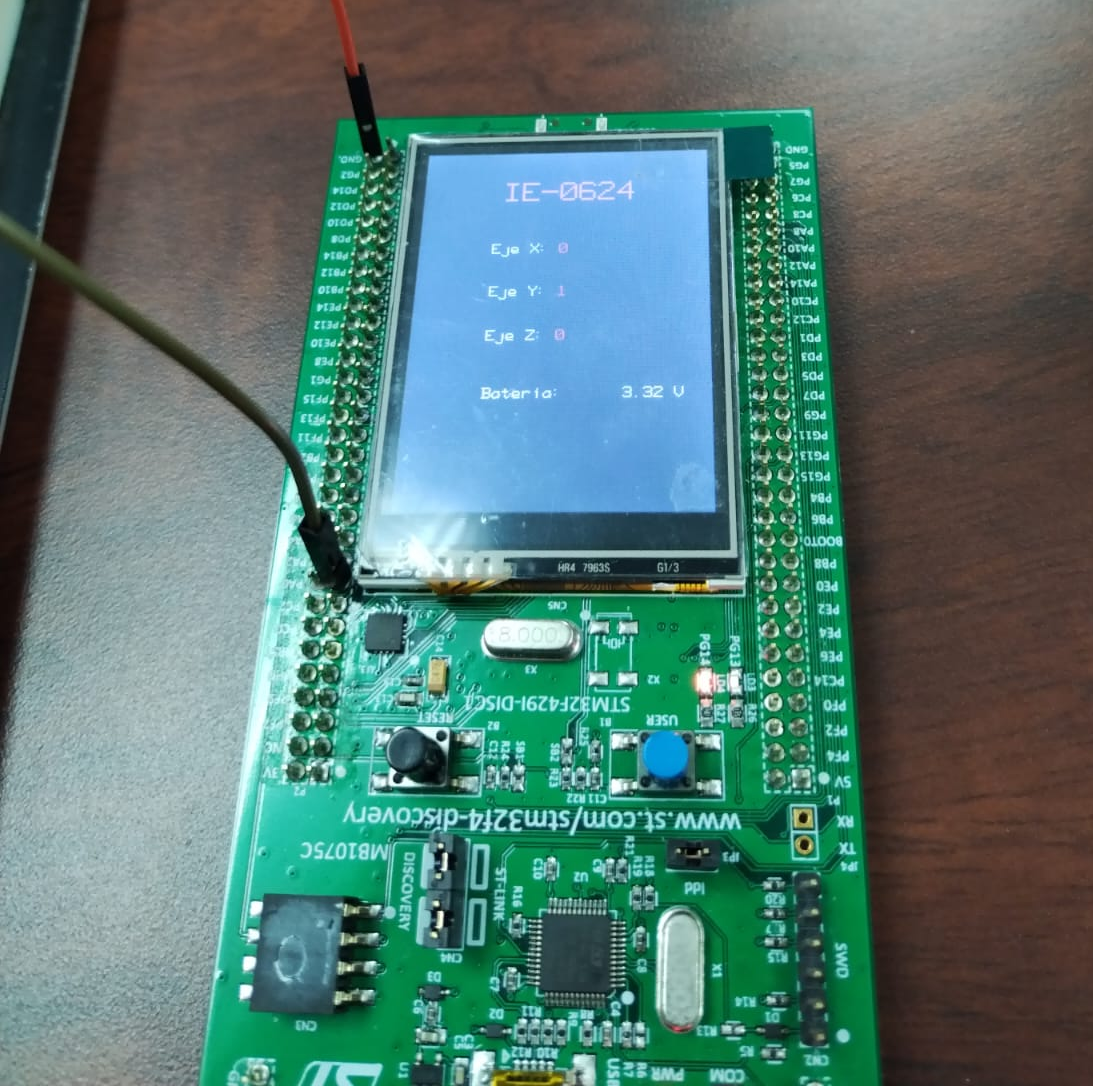
\includegraphics[width=.55\linewidth]{Imagenes/7.png}
 \caption{Magnitud de la batería menor a \SI{7}{\volt}.}
 \label{fig_bat}
\end{figure}
Además, note que de la figura anterior se muestra un LED encendido, lo cual indica una alarma ya que su valor es menor de \SI{7}{\volt}, sino fuera así, entonces el LED no debe encenderse.
\begin{figure}[H]
\centering
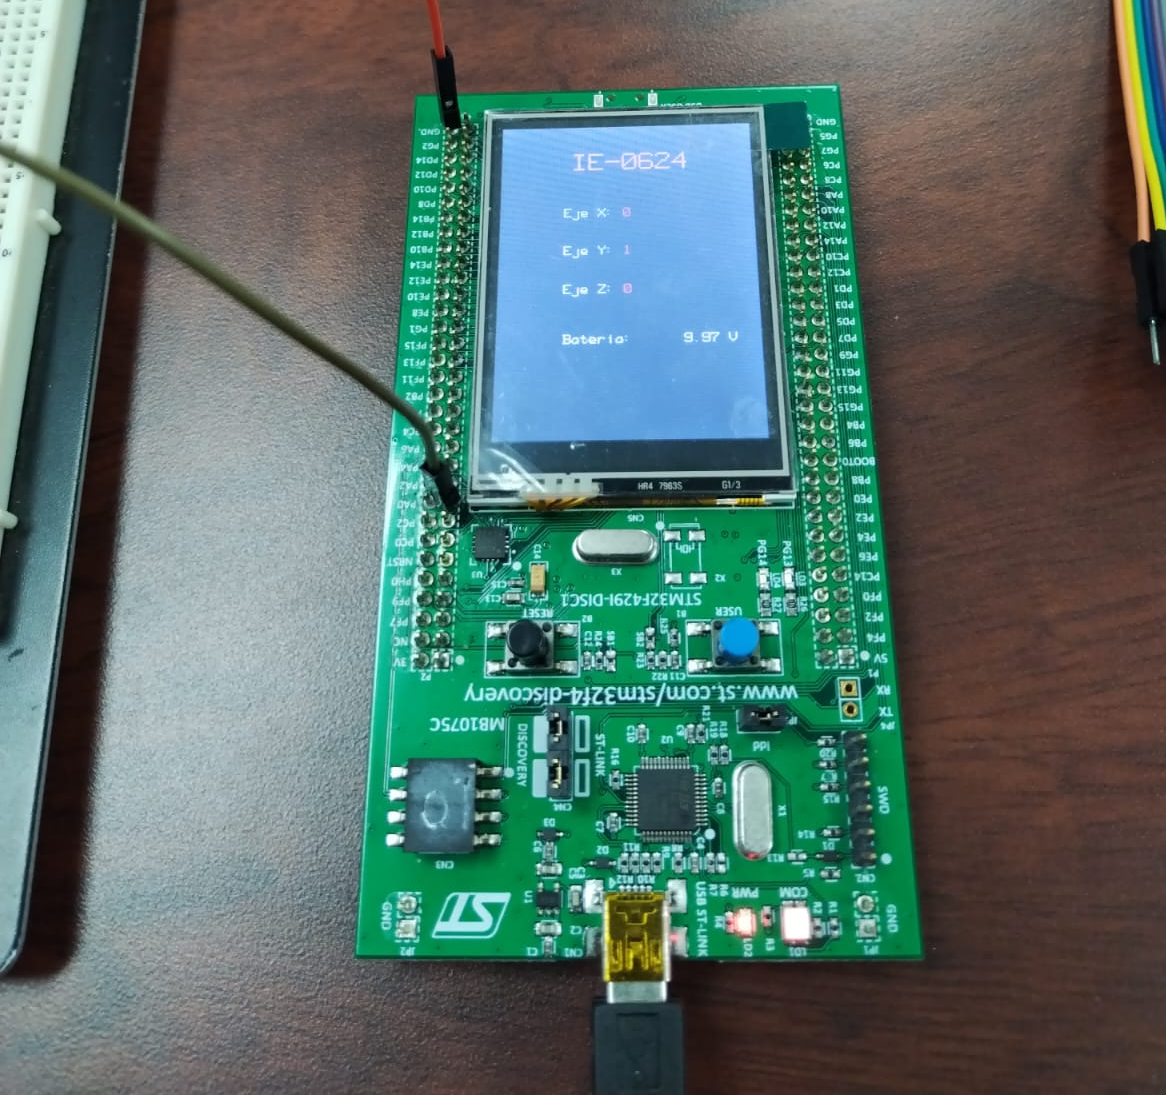
\includegraphics[width=.55\linewidth]{Imagenes/8.png}
 \caption{Magnitud de la batería mayor a \SI{7}{\volt}.}
 \label{fig_bat_OFF}
\end{figure}
Note que el LED \texttt{PG14} no se enciende, lo cual esta correctamente realizado.

Una vez verificado el funcionamiento explicado anteriormente, se procede a realizar la comunicación solicitada por el enunciado. Para ello se toman los datos que se imprimen en la pantalla y se convierten a un formato de bytes para enviarlos usando un protocolo de usart.
Inicialmente se tuvieron diversos problemas, uno de ellos siendo que parecía que los valores no estaban llegando, sin embargo, lo que sucedió es que la cantidad de tiempo que duraba el script de python para recopilar los datos era tanto que solo se mostraban los valores iniciales, por lo que este se tuvo que reducir. Por el problema mencionado, se hizo que el script de python enviara los valores de forma inmediata al dashboard, dependiendo de la aplicación esto sería una mala implementación porque se envían datos cada vez que se hace una lectura de los registros del giroscopio y quita mucho ancho de banda, para aplicaciones que requieren más precisión esto es una buena práctica. La solución a lo anterior es hacer que la lectura del giroscopio no sea tan seguida y de esta forma, por ejemplo, que el script de python envíe datos cada segundo, pero para introducir un retraso se usa ciclos nop, por lo que aumentar esto mucho hace que el MCU consuma potencia haciendo nada.
Por cuestión de tiempo no se tantearon valores y se deja que se envíen datos en casi tiempo real, el resultado obtenido es el siguiente:
\begin{figure}[H]
    \centering
    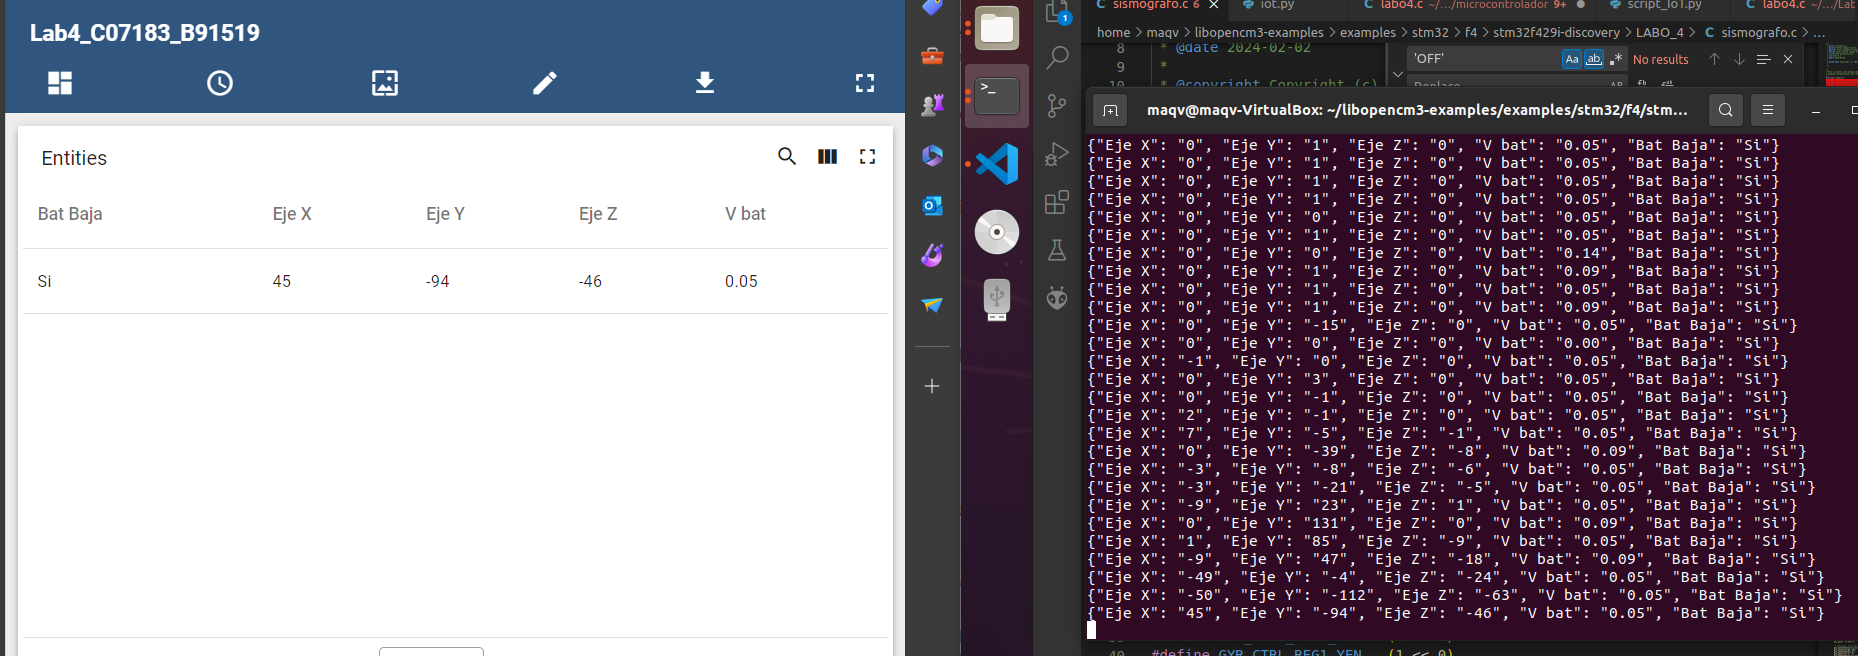
\includegraphics[width=.7\linewidth]{Imagenes/k4.png}
    \caption{Comunicacion con el dashboard y MCU.}
\end{figure}
Se observa el funcionamiento correcto del dashboard también.\\

Cuando se introdujo un retardo en el script se tenía el siguiente resultado, donde se observa que los valores no cambian aún moviendo el giroscopio:
\begin{figure}[H]
    \centering
    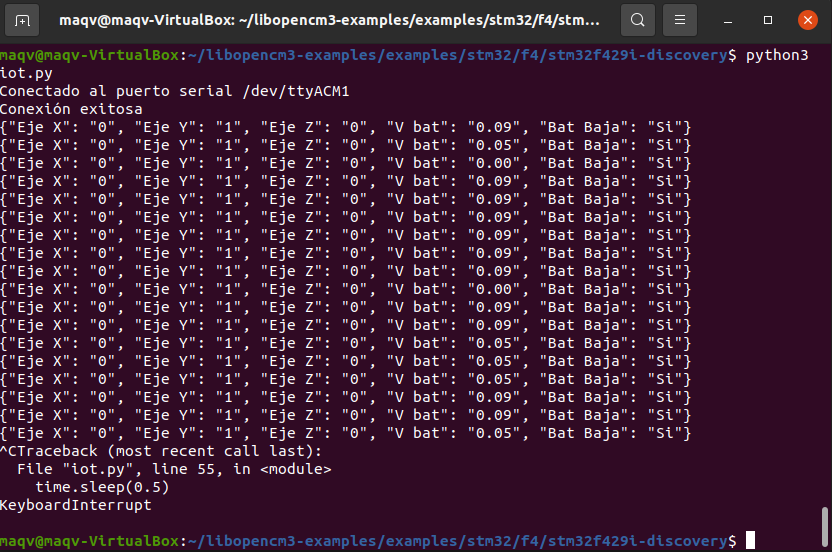
\includegraphics[width=.7\linewidth]{Imagenes/k5.png}
    \caption{Script de python con un retardo.}
\end{figure}

Finalmente se muestra una imagen donde se observa la funcionalidad de todo en conjunto:
\begin{figure}[H]
    \centering
    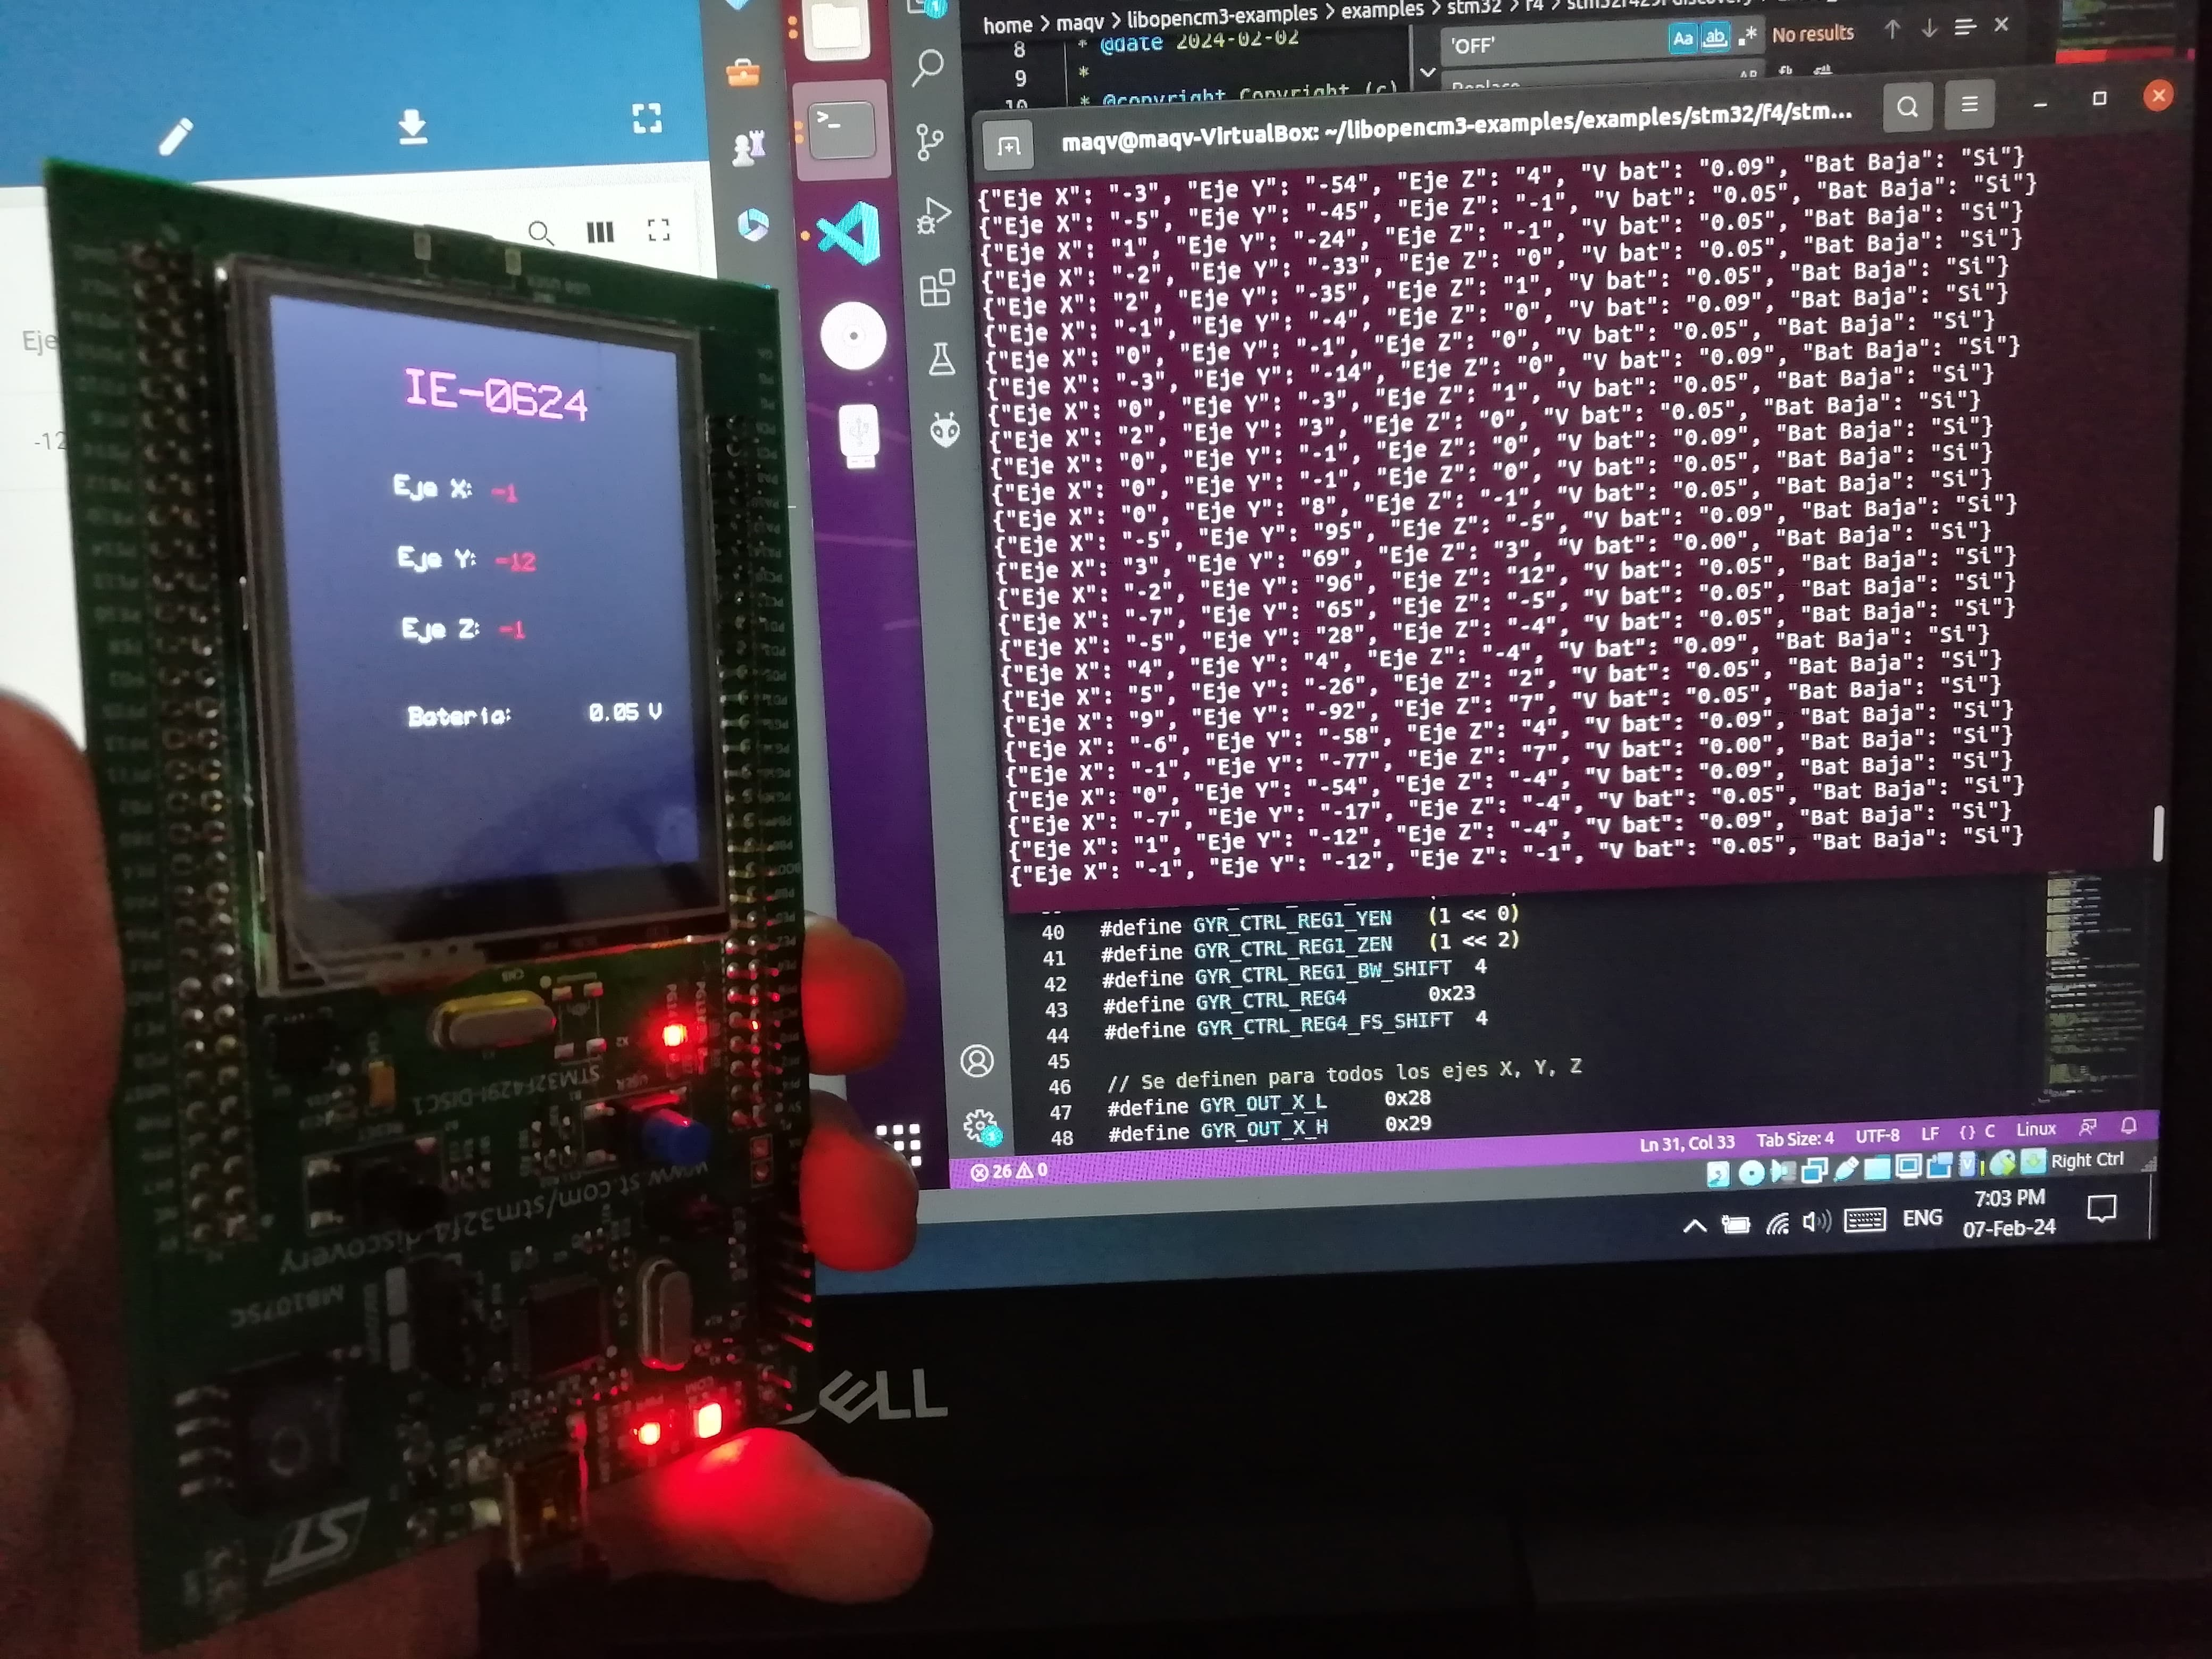
\includegraphics[width=.7\linewidth]{Imagenes/k6.jpg}
    \caption{Giroscopio junto con los datos que se están enviando.}
\end{figure}
Se verifica que los datos se envían correctamente y que el scipt no está saltando valores, también se puede confirmar el funcionamiento con lo que se subió al git, nada mas hay que tener en cuenta que se está utilizando el puerto correcto.\\

La implementación del LED para la comunicación se logró junto con la lógica que se requería para que se habilite/deshabilite la comunicación con un botón, el problema que se tuvo es que el script de python muestra errores cuando no le están llegando datos, una de las posibles soluciones a este problema que se pensó es la implementación de una excepción en python, pero por cuestiones de tiempo no se intentó.
\newpage